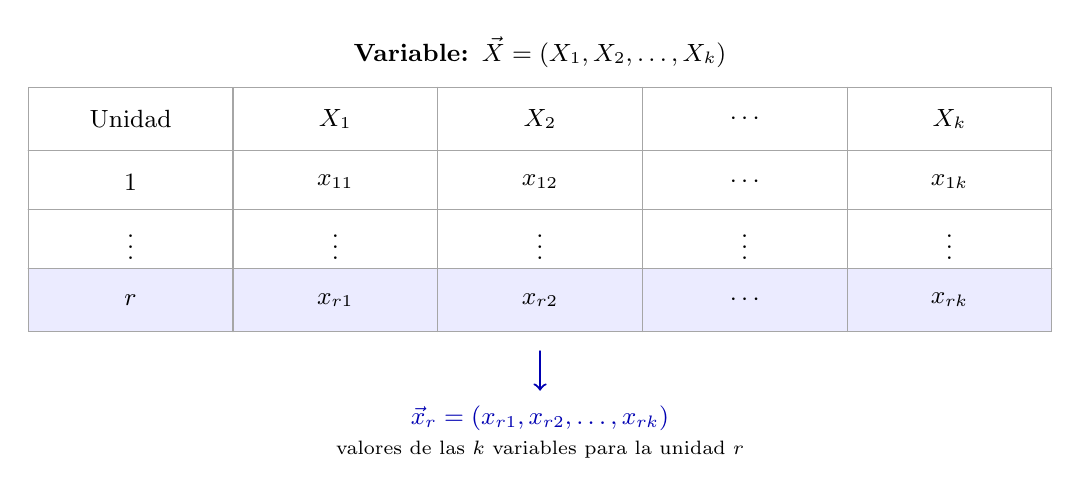
\begin{tikzpicture}[every node/.style={font=\small}, line cap=round]
    % Cada fila representa una unidad y cada columna una variable.
    \node[font=\small\bfseries] at (0,2.35)
        {Variable: $\vec{X}=(X_1,X_2,\ldots,X_k)$};

    % La fila r se destaca para mostrar sus k mediciones.
    \path[fill=blue!8] (-6.5,-1.2) rectangle (6.5,-0.4);
    \draw[gray!70] (-6.5,-1.2) rectangle (6.5,1.9);
    \foreach \x in {-3.9,-1.3,1.3,3.9}
        \draw[gray!70] (\x,-1.2) -- (\x,1.9);
    \foreach \y in {1.1,0.35,-0.4}
        \draw[gray!70] (-6.5,\y) -- (6.5,\y);

    \node at (-5.2,1.5) {Unidad};
    \node at (-2.6,1.5) {$X_1$};
    \node at (0,1.5) {$X_2$};
    \node at (2.6,1.5) {$\cdots$};
    \node at (5.2,1.5) {$X_k$};

    \node at (-5.2,0.7) {$1$};
    \node at (-2.6,0.7) {$x_{11}$};
    \node at (0,0.7) {$x_{12}$};
    \node at (2.6,0.7) {$\cdots$};
    \node at (5.2,0.7) {$x_{1k}$};

    \node at (-5.2,-0.025) {$\vdots$};
    \node at (-2.6,-0.025) {$\vdots$};
    \node at (0,-0.025) {$\vdots$};
    \node at (2.6,-0.025) {$\vdots$};
    \node at (5.2,-0.025) {$\vdots$};

    \node[font=\small\bfseries] at (-5.2,-0.8) {$r$};
    \node[font=\small\bfseries] at (-2.6,-0.8) {$x_{r1}$};
    \node[font=\small\bfseries] at (0,-0.8) {$x_{r2}$};
    \node[font=\small\bfseries] at (2.6,-0.8) {$\cdots$};
    \node[font=\small\bfseries] at (5.2,-0.8) {$x_{rk}$};

    \draw[->,thick,blue!70!black] (0,-1.45) -- (0,-1.95);
    \node[font=\small\bfseries,text=blue!70!black] at (0,-2.3)
        {$\vec{x}_r=(x_{r1},x_{r2},\ldots,x_{rk})$};
    \node[font=\scriptsize] at (0,-2.7) {valores de las $k$ variables para la unidad $r$};
\end{tikzpicture}